% !TEX program = xelatex
% !TEX recipe = xelatex (single run)
\documentclass[10pt,a4paper]{article}

% ===== Page Setup =====
\usepackage[left=1.0cm,right=1.0cm,top=0.7cm,bottom=0.7cm]{geometry}
\usepackage{titlesec}
\usepackage{enumitem}
\usepackage[colorlinks=true,urlcolor=black,linkcolor=black]{hyperref}
\let\oldhref\href
\renewcommand{\href}[2]{\oldhref{#1}{\underline{#2}}}
\usepackage{xcolor}
\usepackage{tabularx}
\usepackage{graphicx}
\usepackage{fontspec}
\setmainfont{Calibri}

% ===== Colors =====
\definecolor{lightgray}{HTML}{666666}
\definecolor{sectioncolor}{HTML}{1A1A1A}

% ===== Spacing =====
\setlength{\parindent}{0pt}
\setlength{\parskip}{0pt}
\pagestyle{empty}
\setlist{nosep}
\linespread{1.2}

% ===== Font Hierarchy =====
% Header: \Large — Name, \normalsize — Contact/Target
% Body (3 levels):
%   Level 1: \normalsize\bfseries — Project titles, school names
%   Level 2: \normalsize — Descriptions
%   Level 3: \normalsize\bfseries — Paper citations (bold)

% ===== Section Style =====
\titleformat{\section}{\large\bfseries\color{sectioncolor}}{}{0em}{}[\vspace{-5pt}\rule{\textwidth}{0.5pt}]
\titlespacing*{\section}{0pt}{20pt}{8pt}

% ===== Custom Commands =====
\newcommand{\project}[3]{%
  \vspace{1pt}
  {\textbf{#1}} {\textbf{(#3)}} \hfill {\color{lightgray}#2}\par\vspace{0pt}
}

\newlength{\projectnumwidth}
\settowidth{\projectnumwidth}{\textbf{[1] }}

\begin{document}

% ===== Header =====
\noindent
\begin{minipage}[c]{0.84\textwidth}
  \centering
  {\Large\bfseries Yecheng Zhang}\\[5pt]
  {
    (+86) 18013979786 (WeChat) \quad$|$\quad
    \href{mailto:zhangyec23@mails.tsinghua.edu.cn}{zhangyec23@mails.tsinghua.edu.cn}\\[2pt]
    \href{https://github.com/24kchengYe}{GitHub} \quad$|$\quad
    \href{https://scholar.google.com/citations?user=6vKhpBoAAAAJ&hl=en}{Google Scholar} \quad$|$\quad
    Preferred: Beijing
  }\\[3pt]
  {\textbf{Target: LLM / AI Algorithm Intern}}
\end{minipage}%
\hfill
\begin{minipage}[c]{0.13\textwidth}
  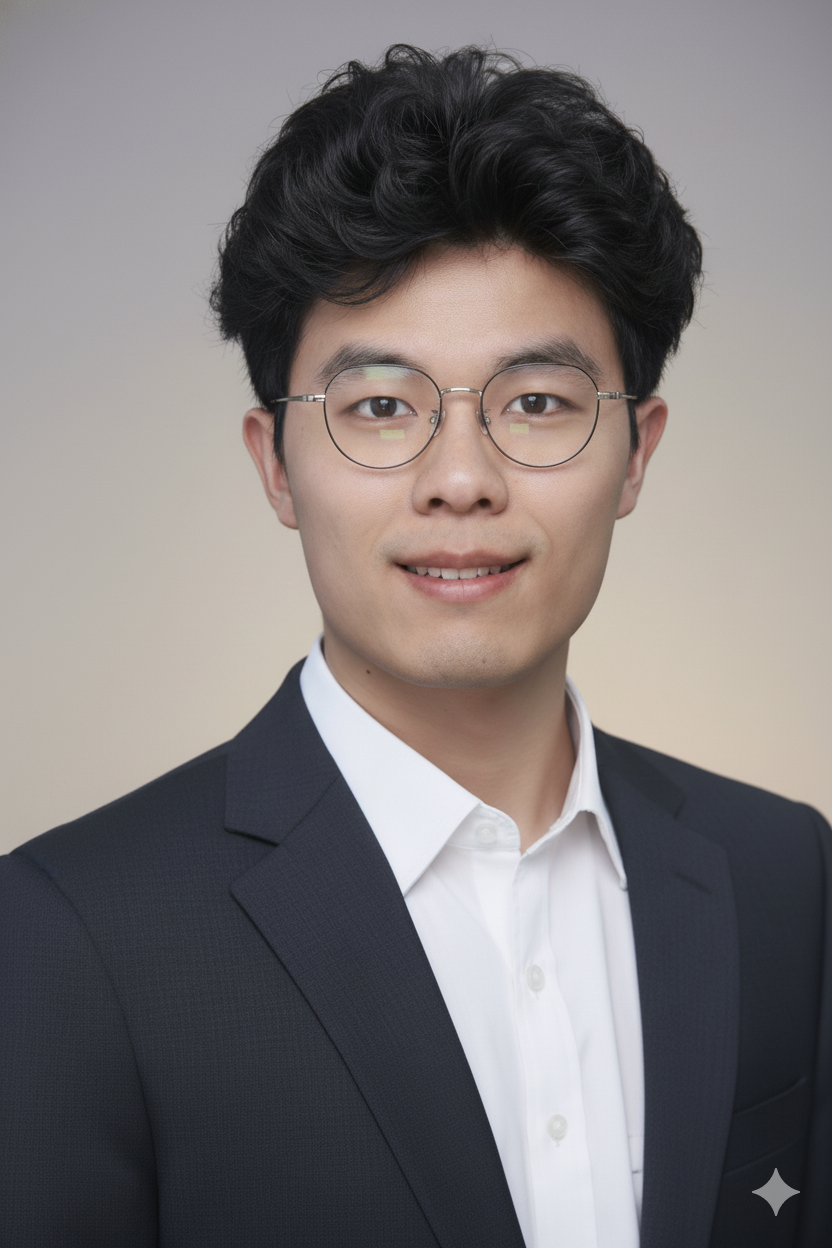
\includegraphics[width=\linewidth, trim=0 2cm 0 0, clip]{photo.png}
\end{minipage}
\vspace{6pt}

% ===== Education =====
\section{Education}

\textbf{Tsinghua University} \hfill 2023.09 -- Present\\
Ph.D. Student in Urban Planning (Research: LLM Evaluation \& Alignment, Urban Science, AI4Science, Computer Vision) $|$ First-Class Scholarship

\vspace{6pt}
\textbf{Hefei University of Technology} \hfill 2018.09 -- 2023.06\\
B.Eng. in Urban Planning $|$ GPA Rank \textbf{1}/40 $|$ Top Ten College Students $|$ Outstanding Graduate

% ===== Research Experience =====
\section{Research Experience}

\project{[1] LLM-Human Preference Alignment via Urban Perception}{2025.10 -- 2026.02}
{First Author $|$ \href{https://arxiv.org/abs/2602.19442}{arXiv} $|$ ECCV 2026 submitted}

\begingroup\leftskip=\projectnumwidth
Large VLMs identify rich visual elements yet remain poorly aligned with human preferences; existing remedies (fine-tuning, RLHF) require labelled data and substantial GPU compute. Proposed a training-free post-hoc concept bottleneck pipeline: automatically discovering interpretable evaluation dimensions, extracting robust concept scores via an Observer-Debater-Judge multi-agent chain from a frozen VLM, and calibrating scores on a hybrid visual-semantic manifold through locally-weighted ridge regression, unified by end-to-end dimension optimization. Achieved \textbf{72.2\%} accuracy ($\kappa$=0.45) on Place Pulse 2.0 across six categories, \textbf{+15.1pp} over supervised baselines, \textbf{+16.3pp} over uncalibrated VLM, with full interpretability and zero weight modification.\\[2pt]
{Paper: \textbf{Zhang Y}, Zhao R, \ldots, Shi C*. UrbanAlign: Post-hoc Semantic Calibration for VLM-Human Preference Alignment. \href{https://arxiv.org/abs/2602.19442}{arXiv}, 2026.}\par
\endgroup

\vspace{12pt}
\project{[2] Evaluating LLM Scientific Data Synthesis}{2024.09 -- 2025.10}
{First Author $|$ \href{https://arxiv.org/abs/2505.13803}{arXiv} $|$ Nature Cities 2nd review}

\begingroup\leftskip=\projectnumwidth
LLMs are increasingly used for scientific data generation, yet their ability to faithfully reproduce complex scientific patterns remains unevaluated. Designed AI4US benchmark evaluating leading international LLMs (GPT, Claude, GLM, DeepSeek, etc.) over \textbf{40K+} synthesis trials across symbolic reasoning and multimodal perception, fitting established scientific laws (scaling laws, distance decay, urban vitality, urban perception). Discovered the \textbf{``group flattening'' effect}, \textbf{systematic bias in fitting established scientific laws}, and \textbf{proposed multi-paradigm prompt optimization strategies} (independent/joint sampling, in-context prompting).\\[2pt]
{Paper: \textbf{Zhang Y}, Zhao R, Huang Z, Long Y*. GenAI Models Capture Urban Science but Oversimplify Complexity. \href{https://arxiv.org/abs/2505.13803}{arXiv}, 2025.}\par
\endgroup

\vspace{12pt}
\project{[3] AI Applications $|$ Global-Scale Urban Open Datasets}{2021.09 -- 2025.10}
{Co-first / First Author $|$ \href{https://doi.org/10.1038/s41597-025-04730-5}{Scientific Data}, \href{https://doi.org/10.1016/j.habitatint.2025.103350}{Habitat International}, \href{https://doi.org/10.1016/j.jag.2022.102942}{JAG}, \href{https://doi.org/10.1016/j.isci.2024.110125}{iScience}}

\begingroup\leftskip=\projectnumwidth
Urban research lacks standardized large-scale urban and building datasets. First, proposed a GAN-based framework fusing multi-source data for urban spatial feature prediction. Then, built global urban boundary dataset GloPPRUA and Global Ghost City Index (GloGCI) via GIS model builder, fusing population, road, and economic data, covering \textbf{8,000+ cities globally}. Finally, built CMAB (China's Multi-Attribute Building Dataset), \textbf{integrating billions of remote sensing and street-view images}, with OCRNet segmentation and XGBoost, covering \textbf{32M+} buildings and \textbf{100+} attributes nationwide. CMAB paper achieved \textbf{ESI Highly Cited} (Geoscience) within six months; data and code \href{https://figshare.com/authors/Yecheng_Zhang/20402873}{\textbf{received 23,000+ downloads}}.\\[2pt]
{Paper: \textbf{Zhang Y}$^{\dag}$, Zhao H$^{\dag}$, Long Y*. CMAB: A Multi-Attribute Building Dataset of China. \href{https://doi.org/10.1038/s41597-025-04730-5}{Scientific Data}, 2025.\\
Paper: \textbf{Zhang Y}, Tu T, Long Y*. Inferring Ghost Cities on the Globe in Newly Developed Urban Areas Based on Urban Vitality with Multi-source Data. \href{https://doi.org/10.1016/j.habitatint.2025.103350}{Habitat International}, 2025.\\
Paper: \textbf{Zhang Y}, Zhang Q, \ldots, Zheng H*. Urban Spatial Risk Prediction and Optimization Analysis of POI Based on Deep Learning. \href{https://doi.org/10.1016/j.jag.2022.102942}{International Journal of Applied Earth Observation and Geoinformation}, 2022.\\
Paper: Li W$^{\dag}$, \textbf{Zhang Y}$^{\dag}$, Li M, Long Y*. Rethinking the Country-Level Percentage of Population Residing in Urban Area with a Global Harmonized Urban Definition. \href{https://doi.org/10.1016/j.isci.2024.110125}{iScience}, 2024.}\par
\endgroup

% ===== Internship Projects =====
\section{Internship Projects}

\project{Municipal Construction Intelligent Bidding System}{2026}
{Solo Developer}

Municipal construction bidding involves qualification review, scoring criteria analysis, and document drafting---manual workflows are inefficient and error-prone. Independently designed a two-stage multi-agent system: the review stage deploys \textbf{7} parallel agents (ThreadPoolExecutor, isolated connection pools) for structured tender analysis (qualification, scoring, risk, etc.); the generation stage uses a Writer$\to$Reviewer$\to$Designer conditionally-triggered pipeline (Designer activates only when Reviewer score falls below threshold), with full agent trace logging. Tech stack integrates ChromaDB RAG, PyMuPDF/RapidOCR parsing (incl. scanned OCR), and \textbf{12+} LLMs with context-window-adaptive model selection, built on Streamlit with \textbf{7,000+} lines of production code. System has produced \textbf{500+} bidding documents for a client company.\par

\vspace{12pt}
\project{Nanjing NUIST Meteorological Science \& Technology Institute}{2025}
{Doctoral Practice $|$ Excellent Evaluation}

Ground-based radar networks have coverage gaps in remote regions (e.g., Xinjiang), limiting real-time severe weather monitoring. Systematically benchmarked \textbf{10+} deep learning architectures (CNN/GAN/Diffusion/Transformer/Flow Matching) for FY-4B satellite-to-radar composite reflectivity inversion using \textbf{22}-channel input (15 base + 7 hand-crafted BTD features encoding cloud phase and moisture gradients); designed exponentially-weighted loss to address extreme class imbalance (severe echoes $<$0.1\% of pixels). Conditional Flow Matching (CFM) achieved CSI \textbf{+7.2\%} and FAR \textbf{-30\%} over baseline; \textbf{zero-shot geographic transfer} to radar-blind Xinjiang validated with GPM satellite data.\\[2pt]
{Paper: Shi C, Han X, \textbf{Zhang Y}, Wu B, Hou J, Wang J, Niu D. AWFlowS2R: A Flow-Based New Paradigm for All-Weather Satellite-to-Radar Retrieval. arXiv, 2026.\\
Paper: Shi C, \ldots, \textbf{Zhang Y}, Niu D. WaveC2R: Wavelet-driven Coarse-to-refined Hierarchical Learning for Radar Retrieval. \href{https://arxiv.org/abs/2511.17558}{AAAI}, 2025.}\par

% ===== Tools & Skills =====
\section{Tools \& Skills}

\begin{tabularx}{\textwidth}{@{}lX@{}}
\textbf{AI/ML} & PyTorch and mainstream DL frameworks, AI coding agents \\
\textbf{Programming} & Python; PyCharm, VS Code; Git; developed skills such as claude-code-recall\\
\textbf{Data} & GIS software \& libraries (QGIS, ArcGIS, GeoPandas, etc.) \\
\end{tabularx}

% ===== Funded Projects =====
\section{Funded Projects}

\begin{itemize}[leftmargin=1.2em, itemsep=3pt, parsep=1pt, topsep=2pt]
  \item NSFC Major Program (No. 62394335, 62394331): Data-Intelligence Driven Urban Agglomeration Resilience Planning
  \item NSFC General Program (No. 52178044): Intelligent Measurement of Urban Vacancy under Shrinkage
  \item Energy Foundation (No. G-2306-34815): Urban Housing Vacancy Measurement and Carbon Emission Implications
\end{itemize}

% ===== Honors =====
\section{Honors}

\begin{itemize}[leftmargin=1.2em, itemsep=3pt, parsep=1pt, topsep=2pt]
  \item National GIS Rising Star (10 awardees), Session Chair of Rising Star Forum, 13th China College GIS Forum, 2025
  \item ``Academic Rising Star'' Nominee (44 university-wide), Tsinghua University, 2025
  \item Outstanding Case Award for ``AI-Empowered Planning'', Urban Planning Society of China, 2025
  \item 2nd Place, ``Big Data Technology Applications'' Course (co-hosted by Tsinghua EE Dept. \& Meituan), 2024
\end{itemize}

% ===== Social Activities =====
\section{Social Activities}

\begin{itemize}[leftmargin=1.2em, itemsep=3pt, parsep=1pt, topsep=2pt]
  \item Talks: AUM at University of Cambridge, GSCS (Hong Kong), etc.
  \item Reviewer: Nature Cities, Scientific Data, npj Urban Sustainability, Cities, Computers, Environment and Urban Systems, Verixiv
  \item Vice Director, Sports Dept., Tsinghua Graduate Student Union, event promotion \& organization, 2024.09 -- 2025.07
\end{itemize}

\end{document}
